\documentclass[11pt]{beamer}

\usepackage[utf8]{inputenc}
\usepackage[T1]{fontenc}
\usepackage{palatino}

% \useoutertheme{noslidenum}

\usepackage{polski}
\usepackage{subfig}
\usepackage{tikz}
\usepackage{amsmath}

\usetheme{Boadilla}

\title[Rodzina protokołów CIP]{%
	Rodzina protokołów CIP
}

\author[Bończyk, Kaźmieruk, Skibiński]
	{Klaudia Bończyk\\Paweł Kaźmieruk\\Maksymilian Skibiński}

\date{25 stycznia 2022 r.}

\graphicspath{
	{./img/}
}

\captionsetup[subfigure]{labelformat = empty}

%\mode<presentation>
%{
%	\setbeamercovered{transparent}
%	% or whatever (possibly just delete it)
%}

\makeatletter
\setbeamertemplate{footline}
{
  \leavevmode%
  \hbox{%
  \begin{beamercolorbox}[wd=.333333\paperwidth,ht=2.25ex,dp=1ex,center]{author in head/foot}%
    \usebeamerfont{author in head/foot}\insertshortauthor~~\beamer@ifempty{\insertshortinstitute}{}{}
  \end{beamercolorbox}%
  \begin{beamercolorbox}[wd=.333333\paperwidth,ht=2.25ex,dp=1ex,center]{title in head/foot}%
    \usebeamerfont{title in head/foot}\insertshorttitle
  \end{beamercolorbox}%
  \begin{beamercolorbox}[wd=.333333\paperwidth,ht=2.25ex,dp=1ex,center]{date in head/foot}%
    \usebeamerfont{date in head/foot}\insertshortdate{}\hspace*{2em}
%    \insertframenumber{} / \inserttotalframenumber\hspace*{2ex} % DELETED
  \end{beamercolorbox}}%
  \vskip0pt%
}
\makeatother




\begin{document}

\frame{\titlepage}


\begin{frame}{Wstęp}
\begin{itemize}
\item Protokół \textbf{CIP} (\emph{Common Industrial Protocol}) jest otwartym protokołem przemysłowym, który jest rozwijany przez ODVA.
\item \textbf{ODVA} (\emph{Open DeviceNet Vendors Association}) to organizacja zrzeszająca osoby ze świata producentów technologii przemysłowych, której celem są wspólne prace nad CIP i jego zastosowaniami.
\end{itemize}

\medskip

\begin{center}
	\includegraphics[width = 0.3 \linewidth]{odva}
\end{center}
\end{frame}


\begin{frame}{Protokół CIP}
Protokół zajmuje się organizacją danych -- definiuje bogaty zbiór wiadomości i poleceń. W modelu OSI zajmuje
górne warstwy.

% \vspace{0.25cm}
\medskip

\begin{center}
	\includegraphics[width = 0.5 \linewidth]{CIP features}
\end{center}
\end{frame}



\begin{frame}{Protokoły wykorzystujące CIP}
Protokół CIP jest wykorzystywany w następujących protokołach sieciowych:
\begin{itemize}
\item EtherNet/IP,
\item DeviceNet,
\item CompoNet,
\item ControlNet.
\end{itemize}

\medskip

Każdy z tych protokołów różni się realizacją dolnych warstw modelu OSI -- górne są te same i wynikają one z CIP.
\end{frame}


\begin{frame}{Protokoły wykorzystujące CIP}{model OSI}
\begin{center}
	\includegraphics[width = 0.85 \linewidth]{cip-stacks}
\end{center}
\end{frame}


\begin{frame}{CIP}{Budowa}
Protokół korzysta z modelowania obiektowego by opisać:
\begin{itemize}
\item zestaw możliwych operacji,
\item sposób w jaki widziane są urządzenia w sieci,
\item uniwersalny sposób na przesył informacji w sieci.
\end{itemize}
\end{frame}


\begin{frame}{CIP}{Węzeł}
Każdy węzeł (\emph{CIP node}) w sieci jest modelowany jako zbiór obiektów. Obiekty są pewną abstrakcyjną
reprezentacją jakiejś informacji czy części urządzenia. Obiekty wspólnie należą do pewnych klas.

\medskip

\begin{center}
	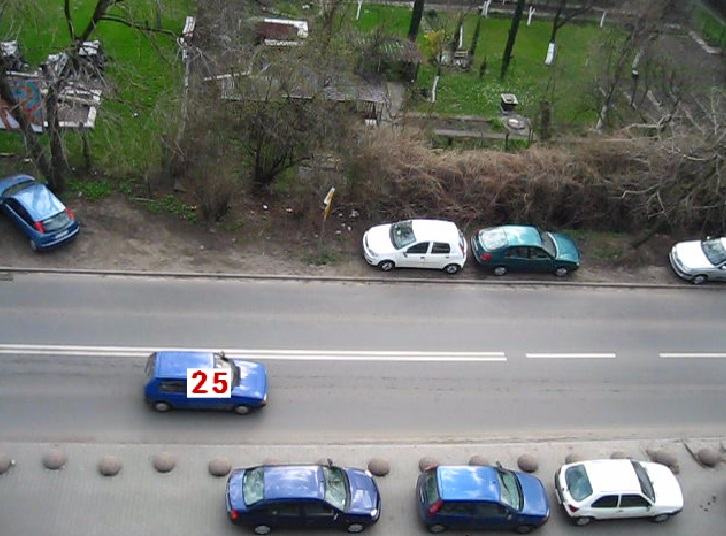
\includegraphics[width = 0.5 \linewidth]{img5}
\end{center}
\end{frame}


\begin{frame}{CIP}{Obiekt}
Na każdy obiekt składają się:
\begin{itemize}
\item dane (\emph{data}),
\item metody/usługi (\emph{services}),
\item połączenia (\emph{connections}),
\item zachowania (\emph{behaviors}) -- relacja pomiędzy danymi, a metodami.
\end{itemize}
\end{frame}


\begin{frame}{CIP}{Obiekt}
Na adresowanie obiektów składa się kilka identyfikatorów:
\begin{itemize}
\item adres węzła,
\item ID klasy,
\item ID obiektu (konkretnego wywołania pewnej klasy),
\item ID atrybuty,
\item kod usługi.
\end{itemize}

\medskip

Wszystkie te identyfikatory są liczbami całkowitymi.
\end{frame}


\begin{frame}{CIP}{Obiekt}
\begin{center}
	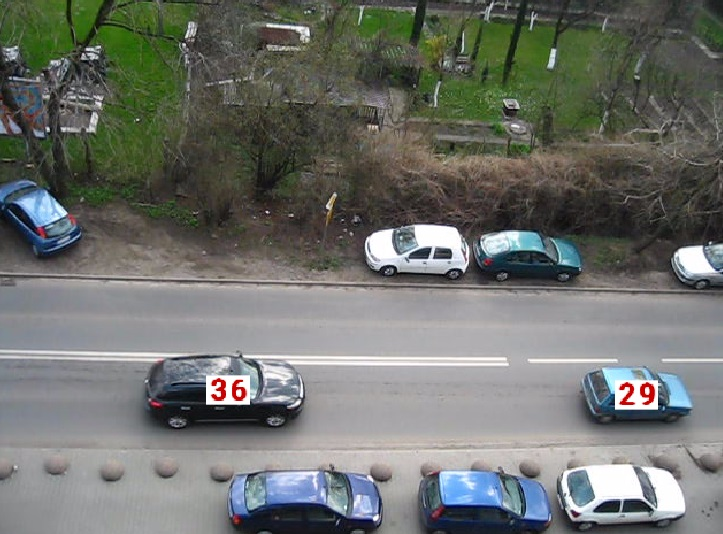
\includegraphics[width = 0.75 \linewidth]{img6}
\end{center}
\end{frame}


\begin{frame}{CIP}{Wiadomości}
Są 2 rodzaje wiadomości:
\begin{itemize}
\item \emph{explicit} -- zawierają takie informacje, które nakazują urządzeniu odbierającemu wykonanie pewnej akcji,
\item \emph{implicit} -- nie zawierają takich informacji, urządzenie odbierające samo wie co zrobić z danymi.
\end{itemize}
\end{frame}


\begin{frame}{CIP}{Wiadomości}

Gdy dochodzi do komunikacji pomiędzy dwoma urządzeniami, połączeniu przypisywane jest ID (CID). Jeśli komunikacja zachodzi w obie strony, wtedy dwa CID zostają przypisane.

\medskip

\begin{center}
	\includegraphics[width = 0.75 \linewidth]{img7}
\end{center}
\end{frame}


\begin{frame}{CIP}{Biblioteka obiektów}
Rodzina protokołów CIP zawiera bogaty zbiór obiektów, które realizują różne operacje. Dzielą się one na trzy rodzaje:
\begin{itemize}
\item zastosowania ogólnego (\emph{general use}),
\item zastosowań szczególnych (\emph{application specific}),
\item zastosowań sieciowych (\emph{network specific}).
\end{itemize}
\end{frame}


\begin{frame}{CIP}{Profile urządzeń}
Urządzenia można modelować w sieci korzystając z wymienionych wcześniej narzędzi, ale pewne urządzenia działają w podobny sposób. By zapewnić większy porządek, takie urządzenia są grupowane za pomocą pewnych profili. Te profile już posiadają pełny opis za pomocą obiektów i zachowań.
\end{frame}


\begin{frame}{CIP}{Typy danych}
Używane typy danych pozostają w zgodzie z normą IEC 61131-3.

Często używane typy to:
\begin{itemize}
\item 1-bitowe: \texttt{BOOL},
\item 1-bajtowe: \texttt{BYTE}, \texttt{USINT}, \texttt{SINT},
\item 2-bajtowe: \texttt{WORD}, \texttt{UINT}, \texttt{INT},
\item 4-bajtowe: \texttt{DWORD}, \texttt{UDINT}, \texttt{DINT}.
\end{itemize}
\end{frame}


% % %
% % %	NETWORK ADAPTATIONS OF CIP
% % %

\begin{frame}{Implementacje CIP}
W tej chwili są 4 publicznie dostępne implementacje protokołu CIP:
\begin{itemize}
\item EtherNet/IP,
\item DeviceNet,
\item CompoNet,
\item ControlNet.
\end{itemize}

\medskip

Każdy z nich różni się warstwami niższymi modelu OSI, a łączy je protokół CIP odpowiadający za górne warstwy tego modelu.
\end{frame}

\begin{frame}{DeviceNet}

Protokół:
\begin{itemize}
\item został opracowany przez firmę Allen-Bradley (teraz przejęta przez Rockwell Automation),
\item wykorzystuje komunikację poprzez CAN,
\item stał się otwartą technologią i został oddany ODVA do dalszego rozwoju,
\item jest bardziej popularny w Ameryce Północnej niż w Europie.
\end{itemize}
\end{frame}


\begin{frame}{DeviceNet}{Ramka danych}
Wykorzystywana przez DeviceNet ramka danych jest następująca:
\begin{itemize}
\item ID ma 11 bitów,
\item dane mają 8 bajtów.
\end{itemize}

\medskip

\begin{center}
	\includegraphics[width = 0.85 \linewidth]{devicenet_2}
\end{center}
\end{frame}


\begin{frame}{DeviceNet}{Topologia}

Topologia sieci opiera się na konfiguracji trunkline/dropline. Na magistrali mogą występować odgałęzienia, a ich liczba zależy od prędkości transmisji.

\medskip

\begin{center}
	\includegraphics[width = 0.75 \linewidth]{devicenet_1}
\end{center}

\end{frame}


\begin{frame}{ControlNet}
Kolejny otwarty protokół opracowany przez Rockwell Automation. W roku 2008 dalszy rozwój został powierzony ODVA. Jest to sieć polowa (fieldbus). Jest ona przeznaczona do wysokowydajnych aplikacji pracujących w czasie rzeczywistym.
\end{frame}


\begin{frame}{ControlNet}{Prędkość przesyłu danych}

\begin{center}
	\includegraphics[width = 0.75 \linewidth]{controlnet_1}
\end{center}
\end{frame}


\begin{frame}{ControlNet}{Warstwa fizyczna}

Wykorzystywany jest kabel koncentryczny RG-6 ze złączami BNC.

\begin{center}
	\includegraphics[width = 0.75 \linewidth]{controlnet_2}
\end{center}
\end{frame}


\begin{frame}{ControlNet}{Topologia sieci}

Sieć może wykorzystywać 3 rodzaje topologi.

\begin{center}
	\includegraphics[width = 0.75 \linewidth]{controlnet_3}
\end{center}
\end{frame}


\begin{frame}{ControlNet}{Token ring}

Gdy węzeł otrzyma token, przysyła swoje dane, aż wykona to w całości lub czas na jaki otrzymał token się skończy. Następnie token przekazywany jest dalej.

\begin{center}
	\includegraphics[width = 0.75 \linewidth]{controlnet_4}
\end{center}
\end{frame}


\begin{frame}{EtherNet/IP}
Protokół opracowany przez Rockwell Automation w roku 2000. Następnie przekazany ODVA. Jest to jeden z najczęściej wykorzystywanych protokółów w Stanach Zjednoczonych.

\vspace{0.25cm}

Protokół jest realizacją CIP na sieci Ethernet.
\end{frame}


\begin{frame}{EtherNet/IP}{Wiadomości}

Wyróżnione są dwa rodzaje wiadomości:
\begin{itemize}
\item wiadomości o znaczeniu niekrytycznym (\emph{explicit}) są przesyłane poprzez protokół TCP,
\item wiadomości o znaczeniu krytycznym (\emph{implicit}) są przesyłane poprzez protokół UDP.
\end{itemize}

\medskip

Te drugie mają oczywiście wyższy priorytet.
\end{frame}


\begin{frame}{EtherNet/IP}{CIPsync}
EtherNet/IP wykorzystuje protokół CIPsync, do synchronizacji zegarów czasu rzeczywistego w rozproszonych systemach. Bazuje on na protokole PTP (\emph{Precision Time Protocol}), który jest protokołem typu master-slave.
\end{frame}


\begin{frame}{CompoNet}
Jest to prostsza sieć, której celem jest szybki przesył mniejszych pakietów danych pomiędzy kontrolerami, czujnikami i aktuatorami.

\vspace{0.5cm}

Cechuje ją dosyć prosty schemat połączeń.
Sygnał jest zakodowany według kodu Manchester.
\end{frame}


%\begin{frame}{CompoNet}{Warstwa fizyczna}
%
%Warstwa fizyczna została stworzona specjalnie na potrzeby tego protokołu.
%
%Sygnał jest zakodowany według kodu Manchester.
%
%\begin{center}
%	\includegraphics[width = 0.75 \linewidth]{componet_1}
%\end{center}
%\end{frame}


\begin{frame}{CompoNet}{Ramka danych}

\begin{center}
	\includegraphics[width = 1 \linewidth]{componet_2}
\end{center}
\end{frame}


\begin{frame}{Rozszerzenia}
Poza wymienionymi sieciowymi implementacjami protokołu CIP, ODVA wypracowała także pewne rozszerzenia protokołu:
\begin{itemize}
\item CIP Security,
\item CIP Safety,
\item CIP Motion,
\item CIP Energy,
\item CIP Sync.
\end{itemize}
\end{frame}


\begin{frame}{Zalety rodziny protokołów CIP}

Dla producentów urządzeń uniwersalny protokół CIP pozwala adaptować go do kolejnych ich sieci, przez co mniej czasu i pieniędzy musi zostać przeznaczonych na rozwój w tym kierunku.

\vspace{0.5cm}

Dla użytkowników protokół skraca czas konieczny na naukę. Wystarczy poznać jedną z sieci wykorzystujących CIP, by umieć sprawnie poruszać się w innych.
\end{frame}


\begin{frame}{Źródła}

Bogatą dokumnetację na temat protokołu CIP można znaleźć na stronie ODVA:
\href{https://www.odva.org/technology-standards/document-library/}{https://www.odva.org/technology-standards/document-library/}.

\vspace{0.5cm}

Szczególną uwagę można poświęcić dokumentowi ,,\emph{The Common Industrial Protocol (CIP) and the Family of CIP Networks}''.

\end{frame}

\begin{frame}

\begin{center}
{\LARGE Dziękujemy za uwagę}
\end{center}

\end{frame}

\end{document}